\documentclass[12pt,a4paper]{article}
\usepackage[utf8]{inputenc}
\usepackage[german]{babel}
\usepackage[T1]{fontenc}
\usepackage{amsmath}
\usepackage{amsfonts}
\usepackage{amssymb}
\usepackage{pdflscape}
\usepackage{makeidx}
\usepackage{graphicx}
\usepackage{fancyhdr}
\author{Lukas Hassel, David Schlosser und Stefan Schmidt}
\title{Millikanversuch}
\cfoot{Lukas Hassel, David Schlosser und Stefan Schmidt}
\lhead{Millikanversuch}
\rhead{\thepage}
\begin{document}
\maketitle
\pagestyle{fancy}

% Aufgaben:
% 1.Versuchsbeschreibung
% 2.Fragen aus Vorbereitung
% 3.Tabelle mit Messungen
% 4.eine Ladungsbestimmung von e als Bespiel
% 5.ein Graph mit unseren Ergebnissen UND mit unserer Interpretertion
%    a.Plot 1: x -> Nr. des Tropfen; y -> errechnete Ladung
%    b.Plot 2: x -> Spannung; y -> Aufstiegsgeschwindigkeit
% Wenn fertig -> per mail an daniel.schneider@uni-siegen.de

\section*{Versuchsbeschreibung}
Der Millikan-Versuch besteht aus zwei Platten die in einem gewissen Abstand voneinander übereinander angeordnet sind. Von oben werden Öltropfen zwischen die Platten gesprüht. Durch ein Mikroskop und eine Skala hinter den Platten ist es Möglich die Fallgeschwindigkeit der Öltröpfchen zu messen. Danach wird an den Platten eine Spannung angelegt so das diese wie ein Kondensator wirken und ein elektrisches Feld entsteht. Wenn die Kraftauswirkung des Feldes auf die Öltröpfchen stark genug ist, steigen die Tröpfchen wieder und man kann die Steiggeschwindigkeit messen. Mit diesen beiden Werten ist es möglich den Radius der Tröpfchen auszurechnen. Durch weitere Berechnungen lässt sich die Elementarladung der Tröpfchen bestimmen.
\section*{Fragen aus der Vorbereitung}
\subsection*{a)}
\subsection*{b)}
Für den Schwebefall müssen die Kraft der Gravitation und die Kraft des elektrischen Feldes gleich groß, mit gegenläufiger Wirkrichtung sein.
\[F_g = F_{el}\]
Die Erdanziehungskraft ist definiert als $F_g = m \cdot g$. Die Kraft mit der der Tropfen in Schwebe gehalten wird ist gegeben durch $F_{el} = \frac{U}{d} \cdot 2e$. Da diese Betragsmäßig gleich sein müssen gilt:
\[m \cdot g  = \frac{U}{d}\]
Damit folgt für die Masse: $m = \frac{U}{d \cdot g}$.
\[m_{oel} = \frac{400V \cdot 2 \cdot 1,6 \cdot 10^{-19}C}{9,81\frac{m}{s^2} \cdot 7,62 \cdot 10^{-3}m} = 1,7123\cdot10^{-15}kg\]
\subsection*{c)}
Bei Verlust eines Elektrons wirkt nun nur noch die halbe elektrische Kraft auf den Öltropfen. Die Änderung der Masse des Öltropfens sind hingegen vernachlässigbar klein, weshalb wir im folgenden weiter die gleiche Anziehungskraft der Erde auf Ihn annehmen werden. Damit ist die Erdanziehungskraft, die auf den Tropfen wirkt größer als die ihr entgegen wirkende Kraft durch das elektrische Feld. Daraus folgt nun, dass der Tropfen zu Boden sinkt.
\subsection*{d)}
Ein Magnetfeld wirkt nur dann eine Kraft auf eine elektrische Ladung, wenn die Ladung sich bewegt, oder das Magnetfeld sich ändert. Der Fall könnte somit nicht aufgehalten werden, es wäre jedoch denkbar ihn durch ein magnetisches Feld zu verlangsamen.
\section*{Beispielrechnung Messung 1}
Gemessene Werte: \\
$U = 2000V,		\\
t_f = 7,68s,	\\
t_r = 22,59s,	\\
d = 0,001m 		\\ $
\\
Aus der gemessenen Fallzeit $t_f$ und der Entfernung $d$ lässt sich die Fallgeschwindigkeit $V_f$ mit der Formel $V_f = \frac{d}{t_f}$ errechnen. \\
$V_f = \frac{0,001m}{7,68s} = 1,302 \cdot 10^{-4} \frac{m}{s}$	\\
Analog lässt sich die Steigzeit $V_r$ errechnen. \\
$V_r = \frac{0,001m}{22,59s} = 4,426 \cdot 10^{-5} \frac{m}{s}$ \\
\\ Der unbekannte Radius $r$ des Öltropfens lässt sich mit der Formel $r=\sqrt{(\frac{b}{2p})^{2} + \frac{9 \cdot \eta \cdot V_f}{2\cdot \rho \cdot g}} - \frac{b}{2p}$ berechnen. Dabei ist $b$ eine Korrekturkonstatnte mit $b=8,2 \cdot 10^{-3} Pa \cdot m$, $p$ der barometrische Luftdruck mit $p = 1013,2 hPa$, $\eta$ die Viskosität der Luft mit $\eta = 1,8 \cdot 10^{-5} \frac{Ns}{m^2}$, $\rho$ die Dichte des Öls mit $\rho = 886 \frac{kg}{m^3}$ und $g$ die Erdbeschleunigung mit $g = 9,81\frac{N}{kg}$.
\\
$r=\sqrt{\frac{8,2\cdot10^{-3}Pa\cdot m}{2\cdot 1013,2 hPa}+\frac{9\cdot 1,8\cdot 10^{-5}Ns/m^2 \cdot 1,302 \cdot 10^{-4} m/s}{2\cdot 886kg/m^3 \cdot 9,81N/kg}}-\frac{8,2\cdot 10^{-3}Pa\cdot m}{2\cdot 1013,2 hPa} = 1,0681\cdot 10^{-6}m$
\\ \\
Mit dem nun bekannten Radius lässt sich die Masse $m$ des Öltröpfchens berechenen mit $m=\frac{4}{3}\cdot \pi \cdot r^3 \cdot \rho = \frac{4}{3} \cdot \pi \cdot (1,0681\cdot 10^{-6}m)^3 \cdot 886kg/m^3 = 4,5223\cdot 10^{-15}kg$.
\\ \\
Zur Berechnung der Ladung ist die Letzte Unbekannte die Feldstärke des elektrischen Feldes, die sich mit der Formel $E=\frac{U}{d} = \frac{2000V}{7,62\cdot 10^{-3}m} = 262,47\frac{kV}{m}$ berechnen lässt.
\\ \\
Schlussendlich ergibt sich nun die Ladung des Öltröpfchens mit \\
$q=\frac{m\cdot g \cdot (V_r + V_f)}{E \cdot V_f}=\frac{4,5223 \cdot 10^{-15}kg \cdot 9,81N/kg\cdot (4,426\cdot 10^{-5}m/s + 1,302\cdot 10^{-4}m/s)}{262,47kV/m \cdot 1,302\cdot 10^{-4}m/s}=2,2648 \cdot 10^{-19}C$
\section*{Ergebnis}
\subsection*{Graphen}
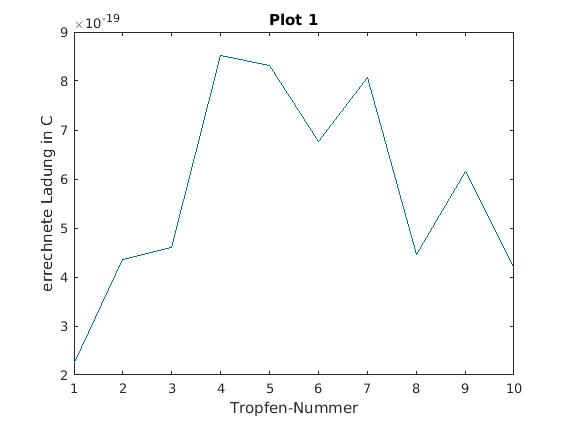
\includegraphics[scale=0.8]{plot1.png}
\\
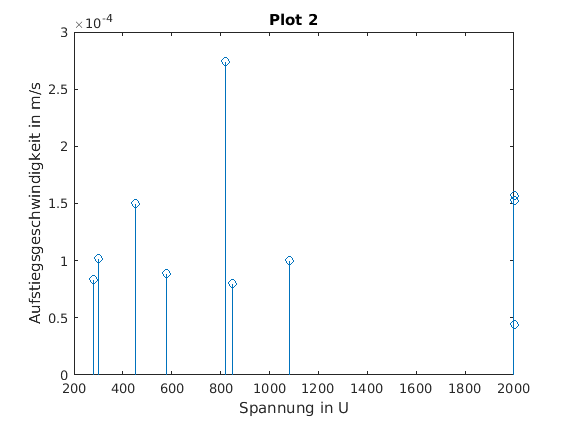
\includegraphics[scale=0.8]{plot2.png}
\begin{landscape}
\section*{Tabelle}
\resizebox{\linewidth}{!}{
\begin{tabular}{c | c | c | c | c | c | c | c}
Messung & Spannung [V]& Fallzeit [s]& Steigzeit [s]& Entfernung [m]& Fallgeschwindigkeit [m/s]& Steiggeschwindigkeit [m/s]& Ladung [C]\\
\hline
\hline
1& 2000 & 7,68 & 22,59 & 0,001 & $1,302\cdot10^{-4}$ & $4,426\cdot10^{-5}$ & $2.2648\cdot10^{-19}$ \\
2& 2000 & 6,38 & 6,57 & 0,001 & $1,567\cdot10^{-4}$ & $1,522\cdot10^{-4}$ & $4.3649\cdot10^{-19}$ \\
3& 2000 & 6,16 & 6,38 & 0,001 & $1,623\cdot10^{-4}$ & $1,567\cdot10^{-4}$ & $4.5944\cdot10^{-19}$ \\
4& 450 & 14,8 & 6,66 & 0,001 & $6,756\cdot10^{-5}$ & $1,502\cdot10^{-4}$ & $8.5197\cdot10^{-19}$ \\
5& 820 & 12,62 & 3,65 & 0,001 & $7,923\cdot10^{-5}$ & $2,739\cdot10^{-4}$ & $8.3074\cdot10^{-19}$ \\
6& 1080 & 6,34 & 9,97 & 0,001 & $1,577\cdot10^{-4}$ & $1,003\cdot10^{-4}$ & $6.7741\cdot10^{-19}$ \\
7& 300 & 18,42 & 9,82 & 0,001 & $5,429\cdot10^{-5}$ & $1,018\cdot10^{-4}$ & $8.0674\cdot10^{-19}$ \\
8& 850 & 10,42 & 12,51 & 0,001 & $9,596\cdot10^{-5}$ & $7,993\cdot10^{-5}$ & $4.4498\cdot10^{-19}$ \\
9& 280 & 23,04 & 11,99 & 0,001 & $4,34\cdot10^{-5}$ & $8,34\cdot10^{-5}$ & $6.1530\cdot10^{-19}$ \\
10& 580 & 16,6 & 11,82 & 0,001 & $6,024\cdot10^{-5}$ & $8,846\cdot10^{-5}$ & $4.2240\cdot10^{-19}$ \\
\end{tabular}}
\end{landscape}
\end{document}
